\documentclass{article}

\usepackage{graphicx}
\usepackage{tikz}
\usepackage{tikzsymbols}
\usetikzlibrary{calc,patterns,shapes.geometric}
\pagestyle{empty}
\usepackage[margin=0pt]{geometry}
\geometry{papersize={14in,12in}}

\def\centerarc[#1](#2)(#3:#4:#5){\draw[#1] ($(#2)+({#5*cos(#3)},{#5*sin(#3)})$) arc (#3:#4:#5);}

\begin{document}
	\begin{figure}
		\centering
		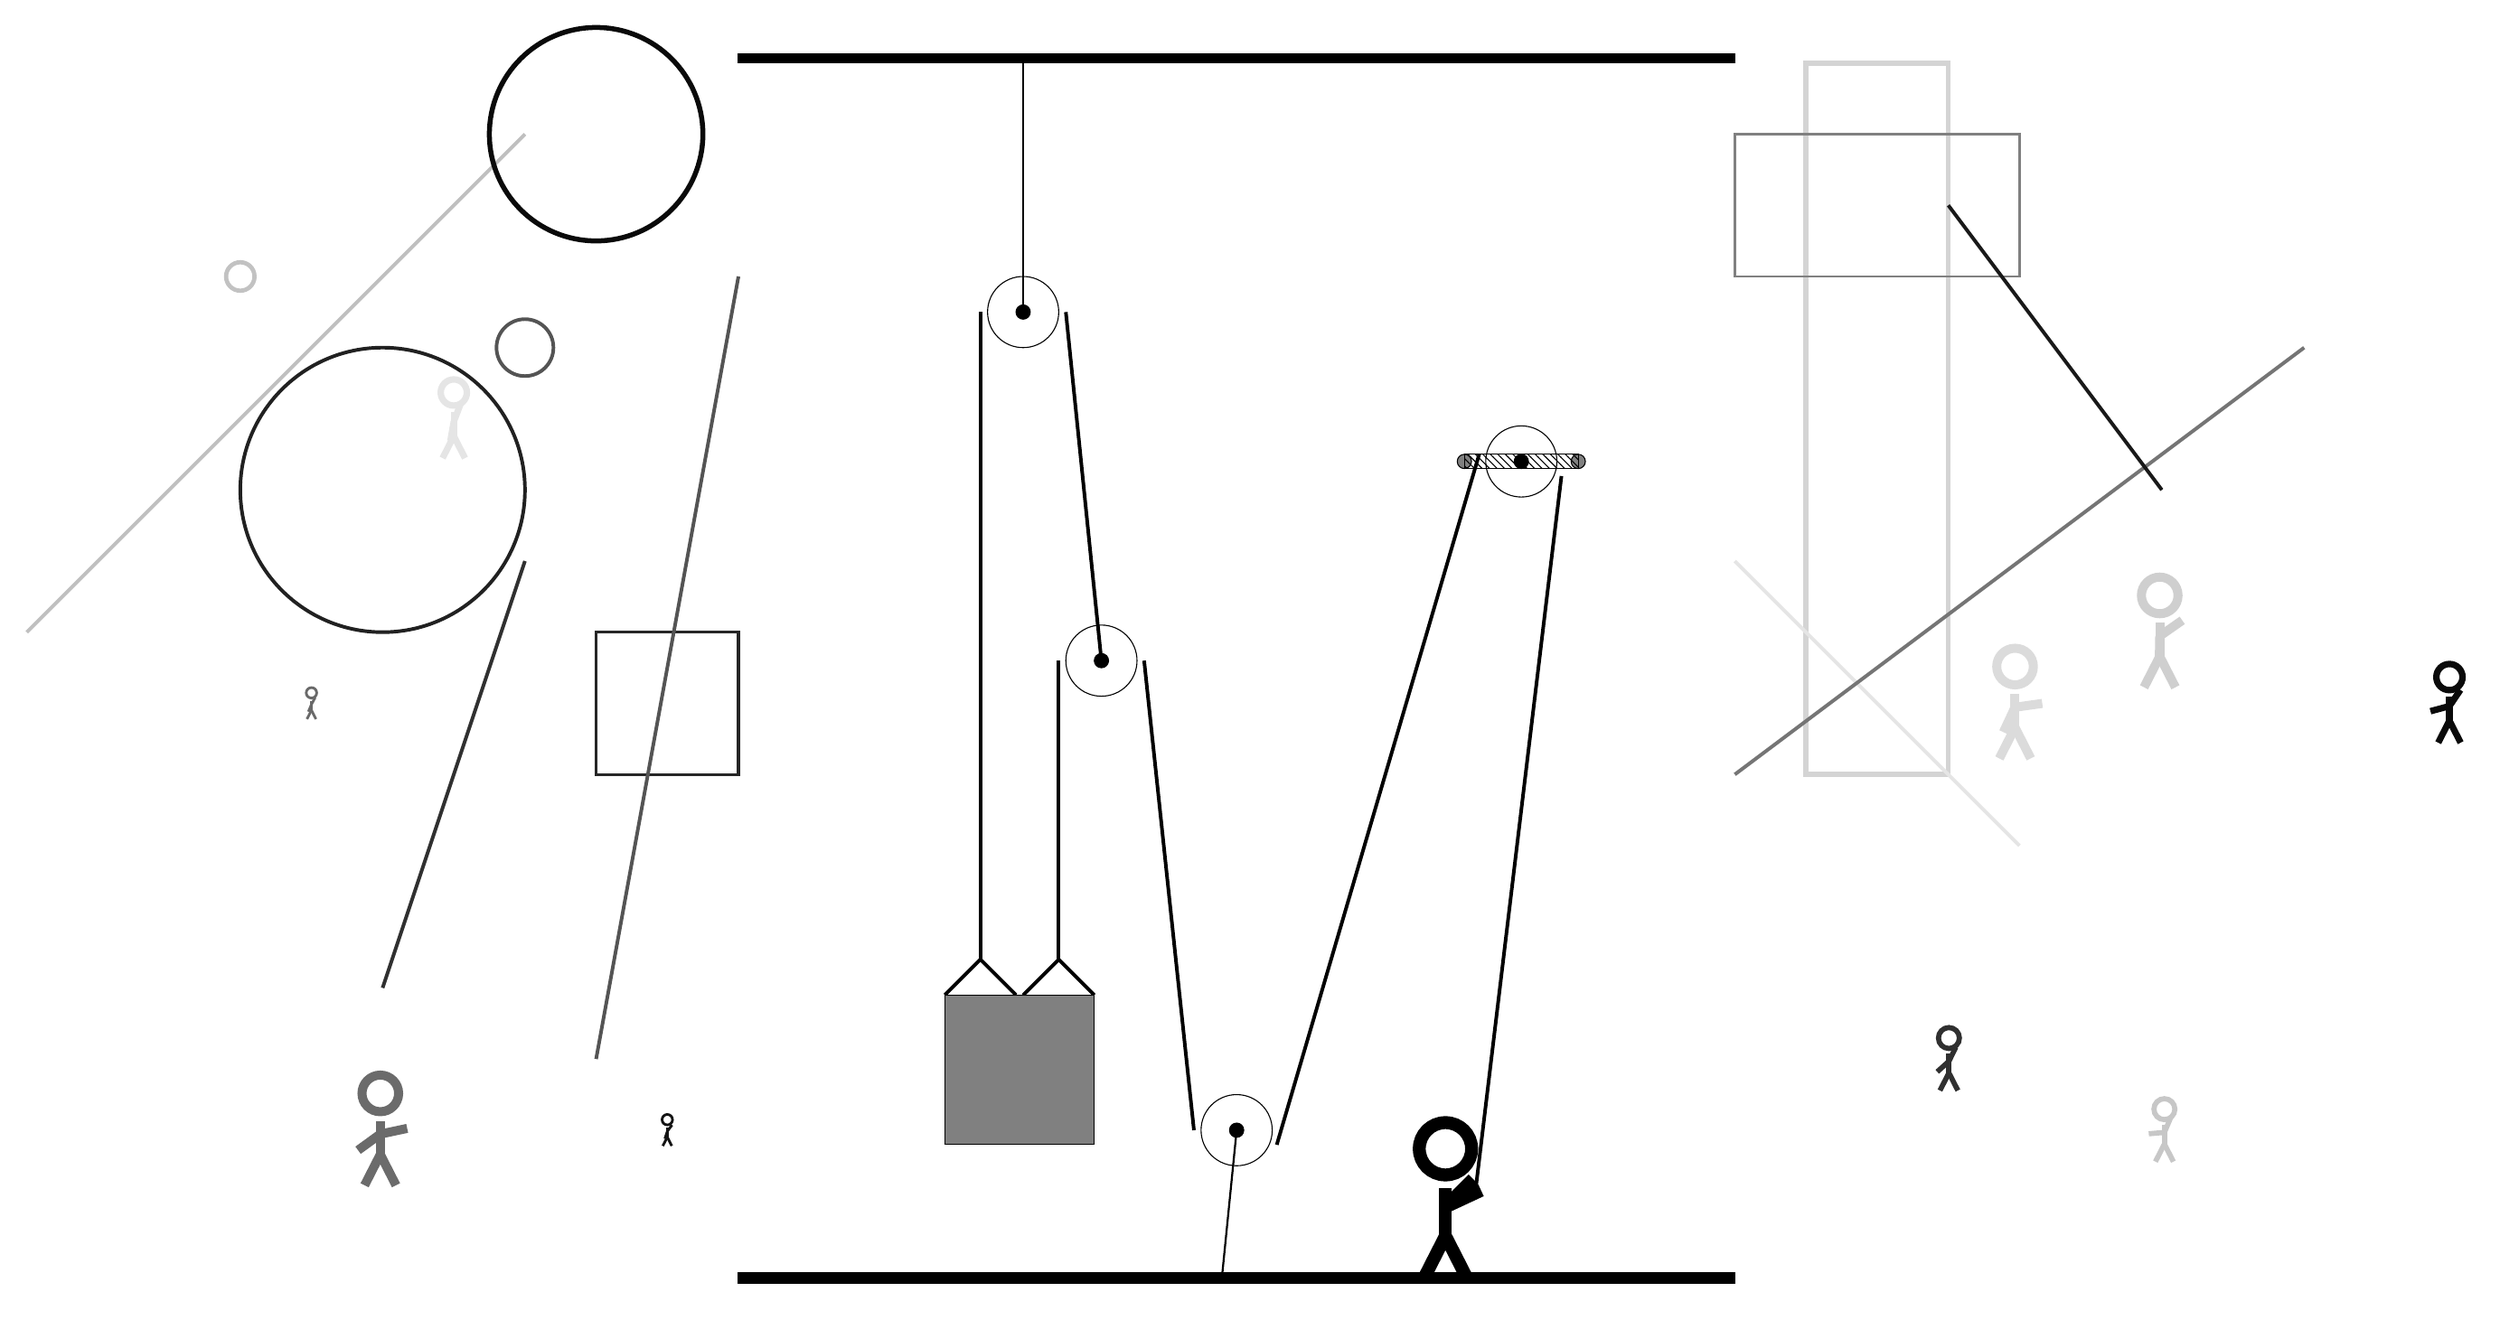
\begin{tikzpicture}
			%%%%% START %%%%%
			
			\draw[fill=black] (-2, 14) rectangle (12, 14.125);
			
			\draw (2, 10.5) circle (0.5);
			\draw[fill=black] (2, 10.5) circle (0.1);
			\draw[thick] (2, 10.5) -- (2, 14);
			
			\draw (3.1, 5.6) circle (0.5);
			\draw[fill=black] (3.1, 5.6) circle (0.1);
			
			\draw (5, -1) circle (0.5);
			\draw[fill=black] (5, -1) circle (0.1);
			\draw[thick] (5, -1) -- (4.8, -3);
			
			\draw (9, 8.4) circle (0.5);
			\draw[fill=black] (9, 8.4) circle (0.1);
			\draw[fill=black!50] (8.2, 8.4) circle (0.1);
			\draw[fill=black!50] (9.8, 8.4) circle (0.1);
			\draw[pattern=north west lines, pattern color=black] (8.2, 8.5) rectangle (9.8, 8.3);
			
			\node[line width=0.3mm, color=black!96] at (22, 5) {\Strichmaxerl[5][15][56]};
			
			\node[line width=0.2mm, color=black!92] at (-3, -1) {\Strichmaxerl[2][72][53]};
			\draw[line width=0.7mm, color=black!17] (13, 4) rectangle (15, 14);
			\draw[line width=0.5mm, color=black!25](-5, 13) -- (-12, 6);
			\draw [line width=0.5mm, color=black!87](-7, 8) circle (2.0);
			\node[line width=0.3mm, color=black!19] at (18, 6) {\Strichmaxerl[7][89][35]};
			\node[line width=0.6mm, color=black!59] at (-8, 5) {\Strichmaxerl[2][67][62]};
			\draw[line width=0.5mm, color=black!81](-5, 7) -- (-7, 1);
			\node[line width=0.2mm, color=black!81] at (15, 0) {\Strichmaxerl[4][42][64]};
			\node[line width=0.6mm, color=black!22] at (18, -1) {\Strichmaxerl[4][5][67]};
			\draw[line width=0.3mm, color=black!50] (12, 13) rectangle (16, 11);
			\draw[line width=0.4mm, color=black!85] (-2, 4) rectangle (-4, 6);
			\draw[line width=0.5mm, color=black!10](16, 3) -- (12, 7);
			
			\node[line width=0.7mm, color=black!10] at (-6, 9) {\Strichmaxerl[5][80][69]};
			\draw [line width=0.7mm, color=black!96](-4, 13) circle (1.5);
			\node[line width=0.2mm, color=black!58] at (-7, -1) {\Strichmaxerl[7][36][12]};
			\draw [line width=0.6mm, color=black!24](-9, 11) circle (0.2);
			\node[line width=0.5mm, color=black!14] at (16, 5) {\Strichmaxerl[7][65][8]};
			\draw [line width=0.5mm, color=black!67](-5, 10) circle (0.4);
			\draw[line width=0.5mm, color=black!67](-2, 11) -- (-4, 0);
			\draw[line width=0.5mm, color=black!54](12, 4) -- (20, 10);
			\draw[line width=0.5mm, color=black!90](15, 12) -- (18, 8);
			
			\draw[line width = 0.5mm]  (0.9, 0.9) -- (1.4, 1.4) -- (1.9, 0.9);
			\draw[line width = 0.5mm]  (2.0, 0.9) -- (2.5, 1.4) -- (3.0, 0.9);
			\draw[fill=black!50] (0.9, 0.9) rectangle (3.0, -1.2);
			
			\draw[line width = 0.5mm] (1.4, 10.5) -- (1.4, 1.4);
			\centerarc[line width = 0.5mm](2, 10.5)(0:180:0.6);
			\draw[line width = 0.5mm] (2.6, 10.5) -- (3.1, 5.6);
			\draw[line width = 0.5mm] (2.5, 5.6) -- (2.5, 1.4);
			\centerarc[line width = 0.5mm](3.1, 5.6)(0:180:0.6);
			\draw[line width = 0.5mm] (3.7, 5.6) -- (4.4, -1);
			\centerarc[line width = 0.5mm](5, -1)(180:340:0.6);
			\draw[line width=0.5mm](5.5638, -1.2052) -- (8.4091, 8.5042);
			\centerarc[line width = 0.5mm](9, 8.4)(-20:170:0.6);
			\draw[line width=0.5mm](9.5638, 8.1948) --  (8.35, -1.9);
			
			\node at (8, -2) {\Strichmaxerl[10][225][25]};
			
			\draw[fill=black] (-2, -3) rectangle (12, -3.15);
			
			%%%%% END %%%%%
		\end{tikzpicture}
	\end{figure}	
\end{document}